\chapter{Annexes}

\section{Témoignages de deux personnes en situation de handicap}

Deux questionnaires ont été soumis à deux personnes handicapées réintégrés professionnellement. Ces deux personnes, issus d'un centre de rééducation fonctionnelle, ont été suivies par l'association Comète pour recouvrer un emploi.\\

Les résultats de ces questionnaires sont assez mitigés car aucune véritable réaction n'a été observée par ces employés. C'est parce qu'ils étaient dans un circuit de réinsertion professionnelle soutenu par l'association Comète que l'insertion et l'intégration se sont bien déroulés. En effet, les entreprises cibles ont été sensibilisées au handicap et, comme le montre les deux questionnaires, l'intégration professionnelle s'est bien déroulée. \\

1. Exercez-vous une activité professionnelle actuellement ?\\
Personne A : Oui - Technicien Analyse BioMédicale.\\
\textit{Tâche} : Analyse de prélèvements de sang, urine, fécales, moelle osseuse dans la recherche de pathologies.\\
Personne B : Oui - Technicien de bureau d'étude en électricité pour le nucléaire.\\ \textit{Tâche} : Conception et réalisation de coffrets et armoires pour la ventilation des centres nucléaires \\


2. Quel a été votre parcours professionnel depuis l’accident?\\
Personne A : BTS et Stage. \\
\textit{Délai de reprise d'activité professionnelle} : 8 mois.\\
\textit{Difficultés rencontrées dans la recherche de l'emploi} : Accessibilité aux locaux, difficultés de structure liées à l'architecture.\\
Personne B : \textit{Délai de reprise d'activité professionnelle} : 4 ans \\ 
\textit{Parcours suivi à la sortie du centre de rééducation} : 
\begin{enumerate}
\item Nécessité de compléter ma formation (avant l’accident, titulaire d’un BEP d’électrotechnique) sur 2 années au CRIP de Castelnau le lez (34) pour me spécialiser en bureau d’études
\item Intégration d’un poste au bout de 4 ans au total après l’accident\\
\end{enumerate}
\textit{Difficultés rencontrées dans la recherche de l'emploi} : Aucune car j'ai été sollicité par l'entreprise sur le lieu de stage ! \\


3. Avez-vous réintégré votre emploi antérieur à l’accident ?\\
Personne A : Non \\
Personne B : Non (pas d'emploi avant l'accident)\\


4. Avez-vous bénéficié d’un accompagnement par une association pour intégrer votre emploi ? \\
Personne A : Oui, par l'association Comète à Propara\\
Personne B : Oui. Recherche de formations et accompagnement par Comète France. Contact établi entre Comète France (département Propara) et le CRIP de Castelnau le lez. \\


5. Avez vous rencontré des difficultés d’intégration dans l’équipe ?\\
Personne A : Non \\
Personne B : Non \\


6. Avez-vous bénéficié d’un aménagement de votre poste de travail ? \\
Personne A : Non \\
Personne B : Non (poste déjà aménagé) \\


7. Avez vous rencontré des problèmes de concrétisation de votre aménagement de poste ou d'accessibilité par l'entreprise ?\\
Personne A : Non \\
Personne B : Non \\




8. Vous êtes vous heurtés à des réactions particulières positives ou négatives de votre entourage professionnelle ?\\
Personne A : Non \\
Personne B : Oui - Réactions plutôt positives de compréhension et volonté d’apporter de l’aide\\


9. Parlez-vous facilement de votre handicap au travail ?\\
Personne A : Oui. \textit{Vous êtes vous heurtés à certains préjugés ou questions déplacées ? } : Ni de préjugés, ni de questions déplacées, de la curiosité plutôt\\
Personne B : Oui \\


10. Êtes-vous interrogé sur votre handicap au travail ?\\
Personne A : Oui\\
Personne B : Oui - Questions relevant de la curiosité sur ce qui m’est arrivé et comment s’est arrivé ?\\



11. Pensez-vous pouvoir évoluer dans votre entreprise ?\\
Personne A : Oui \\
Personne B : Oui \\


12. Y a t-il dans votre entreprise une véritable stratégie d’embauche de personnes en situation de handicap  (autres employés que vous en situation handicap, mission handicap etc.) ?\\
Personne A : Non \\
Personne B : Non \\



\section{Lois}

\subsection{Loi du 10 Juillet 1987}

\begin{figure}
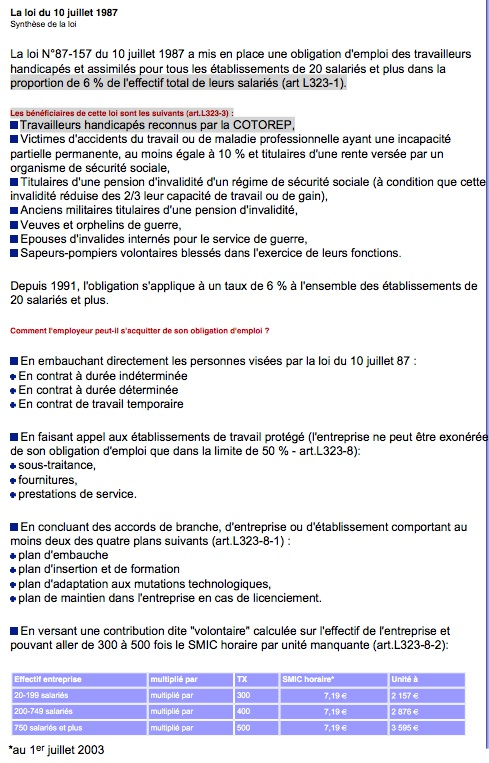
\includegraphics[scale=0.9]{figures/loi_juillet_1987.jpg}
\centering
\end{figure}

\subsection{Loi du 12 Février 2005}

\begin{center}
JORF \no 36 du 12 février 2005 page 2353\\
texte \no 1
\end{center}

\begin{center}
LOI \no 2005-102 du 11 février 2005 pour l'égalité des droits et des chances, la participation et la citoyenneté des personnes handicapées (1)\\
\end{center}


\textbf{Chapitre II : Emploi, travail adapté et travail protégé}\\

\textbf{Section 1 : Principe de non-discrimination}\\

\textbf{Article 23}\\

L'article L. 122-24-4 du code du travail est ainsi modifié :
…..\\

II. - Après l'article L. 122-45-3 du même code, il est inséré un article L. 122-45-4 ainsi rédigé :\\
« Art. L. 122-45-4. - Les différences de traitement fondées sur l'inaptitude constatée par le médecin du travail dans le cadre du titre IV du livre II en raison de l'état de santé ou du handicap ne constituent pas une discrimination lorsqu'elles sont objectives, nécessaires et appropriées.\\
« Les mesures appropriées au bénéfice des personnes handicapées visant à favoriser l'égalité de traitement prévues à l'article L. 323-9-1 ne constituent pas une discrimination. »\\

III. - Après l'article L. 122-45-3 du même code, il est inséré un article L. 122-45-5 ainsi rédigé :\\
« Art. L. 122-45-5. - Les associations régulièrement constituées depuis cinq ans au moins, oeuvrant dans le domaine du handicap, peuvent exercer en justice toutes actions qui naissent des articles L. 122-45 et L. 122-45-4, dans les conditions prévues par l'article L. 122-45, en faveur d'un candidat à un emploi, à un stage ou une période de formation en entreprise ou d'un salarié de l'entreprise, sous réserve qu'elles justifient d'un accord écrit de l'intéressé. Celui-ci peut toujours intervenir à l'instance engagée par l'association et y mettre un terme à tout moment. »\\

IV. - Après l'article L. 323-9 du même code, il est inséré un article L. 323-9-1 ainsi rédigé :\\
« Art. L. 323-9-1. - Afin de garantir le respect du principe d'égalité de traitement à l'égard des travailleurs handicapés mentionnés à l'article L. 323-3, les employeurs prennent, en fonction des besoins dans une situation concrète, les mesures appropriées pour permettre aux travailleurs mentionnés aux 1, 2, 3, 4, 9, 10 et 11 de l'article L. 323-3 d'accéder à un emploi ou de conserver un emploi correspondant à leur qualification, de l'exercer ou d'y progresser ou pour qu'une formation adaptée à leurs besoins leur soit dispensée, sous réserve que les charges consécutives à la mise en oeuvre de ces mesures ne soient pas disproportionnées, compte tenu des aides qui peuvent compenser en tout ou partie les dépenses supportées à ce titre par l'employeur.\\
« Ces aides peuvent concerner notamment l'adaptation de machines ou d'outillages, l'aménagement de postes de travail, y compris l'accompagnement et l'équipement individuels nécessaires aux travailleurs handicapés pour occuper ces postes, et les accès aux lieux de travail.\\
« Le refus de prendre des mesures appropriées au sens du premier alinéa peut être constitutif d'une discrimination au sens de l'article L. 122-45-4. »\\



\textbf{Article 25}\\

I. - L'article L. 132-12 du code du travail est complété par deux alinéas ainsi rédigés :\\
« Les organisations mentionnées au premier alinéa se réunissent pour négocier, tous les trois ans, sur les mesures tendant à l'insertion professionnelle et au maintien dans l'emploi des travailleurs handicapés. La négociation porte notamment sur les conditions d'accès à l'emploi, à la formation et à la promotion professionnelles ainsi que sur les conditions de travail, de maintien dans l'emploi et d'emploi.\\
« La négociation sur l'insertion professionnelle et le maintien dans l'emploi des travailleurs handicapés se déroule sur la base d'un rapport établi par la partie patronale présentant, pour chaque secteur d'activité, la situation par rapport à l'obligation d'emploi des travailleurs handicapés prévue par la section 1 du chapitre III du titre II du livre III. »\\

II. - L'article L. 132-27 du même code est complété par trois alinéas ainsi rédigés :\\
« Dans les entreprises mentionnées au premier alinéa, l'employeur est également tenu d'engager, chaque année, une négociation sur les mesures relatives à l'insertion professionnelle et au maintien dans l'emploi des travailleurs handicapés. La négociation porte notamment sur les conditions d'accès à l'emploi, à la formation et à la promotion professionnelles, les conditions de travail et d'emploi ainsi que les actions de sensibilisation au handicap de l'ensemble du personnel de l'entreprise.\\
« La négociation sur l'insertion professionnelle et le maintien dans l'emploi des travailleurs handicapés se déroule sur la base d'un rapport établi par l'employeur présentant la situation par rapport à l'obligation d'emploi des travailleurs handicapés prévue par la section 1 du chapitre III du titre II du livre III.\\
« A défaut d'une initiative de l'employeur depuis plus de douze mois suivant la précédente négociation, la négociation s'engage obligatoirement à la demande d'une organisation syndicale représentative dans le délai fixé à l'article L. 132-28 ; la demande de négociation formulée par l'organisation syndicale est transmise dans les huit jours par l'employeur aux autres organisations représentatives. Lorsqu'un accord collectif comportant de telles mesures est signé dans l'entreprise, la périodicité de la négociation est portée à trois ans. »\\

III. - Après le mot : « relatives », la fin du 3 de l'article L. 133-5 du même code est ainsi rédigée : \\
« aux diplômes et aux titres professionnels délivrés au nom de l'Etat, à condition que ces diplômes et titres aient été créés depuis plus d'un an ; ».\\

IV. - Au 11 de l'article L. 133-5 du même code, les mots : « prévue à l'article L. 323-9 » sont remplacés par les mots : « prévue à l'article L. 323-1, ainsi que par des mesures d'aménagement de postes ou d'horaires, d'organisation du travail et des actions de formation visant à remédier aux inégalités de fait affectant ces personnes ».\\

V. - Au 8 de l'article L. 136-2 du même code, après les mots : « ou une race, », sont insérés les mots : « ainsi que des mesures prises en faveur du droit au travail des personnes handicapées, ».\\

VI. - Dans le III de l'article 12 de la loi \no 2003-775 du 21 août 2003 portant réforme des retraites, les mots : « à l'avant-dernier » sont remplacés par les mots : « au septième ».\\


\textbf{Section 2 : Insertion professionnelle et obligation d'emploi}\\


\textbf{Article 26}\\

…
III. - L'article L. 323-11 du même code est ainsi rédigé :\\
« Art. L. 323-11. - Des centres de préorientation contribuent à l'orientation professionnelle des travailleurs handicapés.
« Des organismes de placement spécialisés en charge de la préparation, de l'accompagnement et du suivi durable dans l'emploi des personnes handicapées participent au dispositif d'insertion professionnelle et d'accompagnement particulier pendant la période d'adaptation au poste de travail des travailleurs handicapés mis en oeuvre par l'Etat, le service public de l'emploi, l'association mentionnée à l'article L. 323-8-3 et le fonds visé à l'article L. 323-8-6-1. Ils doivent être conventionnés à cet effet et peuvent, à cette condition, recevoir l'aide de l'association et du fonds susmentionnés.\\

IV. - Dans le 2 de l'article L. 381-1 et le 5 de l'article L. 542-1 du code de la sécurité sociale, les mots : « L. 323-11 du code du travail » sont remplacés par les mots : « L. 241-5 du code de l'action sociale et des familles ».
V. - Après l'article L. 323-11 du code du travail, il est inséré un article L. 323-11-1 ainsi rédigé :\\
« Art. L. 323-11-1. - L'Etat, le service public de l'emploi, l'association visée à l'article L. 323-8-3, le fonds visé à l'article L. 323-8-6-1, les conseils régionaux, les organismes de protection sociale, les organisations syndicales et associations représentatives des personnes handicapées définissent et mettent en oeuvre des politiques concertées d'accès à la formation et à la qualification professionnelles des personnes handicapées qui visent à créer les conditions collectives d'exercice du droit au travail des personnes handicapées.\\
« Ces politiques ont pour objectif de recenser et quantifier les besoins de formation des personnes handicapées ainsi que la qualité des formations dispensées. Elles favorisent l'utilisation efficiente des différents dispositifs en facilitant la mise en synergie entre les organismes de formation ordinaires et les organismes spécialement conçus pour la compensation des conséquences du handicap ou la réparation du préjudice.\\
« En vue de garantir une gamme complète de services aux personnes handicapées tenant compte de l'analyse des besoins en respectant notamment la possibilité de libre choix de ces personnes et également en tenant compte de la proximité des lieux de formation, une programmation pluriannuelle de l'accueil en formation est prévue.\\
« Afin de tenir compte des contraintes particulières des personnes handicapées ou présentant un trouble de santé invalidant, un accueil à temps partiel ou discontinu, une durée adaptée de la formation et des modalités adaptées de validation de la formation professionnelle sont prévus dans des conditions fixées par décret. »